\section{Watchdogs}

A watchdog timer is basically an internal or external device (timer) that is installed in a system in order to detect any software anomalies that may arise in embedded systems.
It has the responsibility to reset and restart the processor when needed in the case of a software glitch.
It is also called Computer Operating Properly (COP).

With billions of IoT devices being deployed in the field, it
would be impossible for a technician to service them in a
timely manner if something goes wrong
– IoT systems must be able to detect and recover from faults on their
own without any human intervention
 Watchdogs come in many different shapes and sizes, but
can generally be categorized as simple timers, windowed
timers and smart watchdogs
– Watchdogs may exist internally to microcontrollers as hardware and
software, externally as hardware, and even as separate
microcontrollers with both hardware and software components
– No matter which watchdog solution is used, the sole purpose is to
monitor and recover the system. To this end, each watchdog has its
own unique characteristics and design challenges that developers
need to consider for a robust IoT system

\subsection{Workflow}
Normally the computer regularly resets the watchdog timer to prevent it from elapsing, or "timing out“
In the case of hw fault or program error, the computer fails to reset the watchdog, the timer will elapse and generate a timeout signal
The timeout signal initiates corrective actions (not always RESET!!!)
The corrective actions typically include placing the computer system in a safe state and restoring normal system operation

\subsection{Architecture}
\begin{figure}[H]
    \centering
    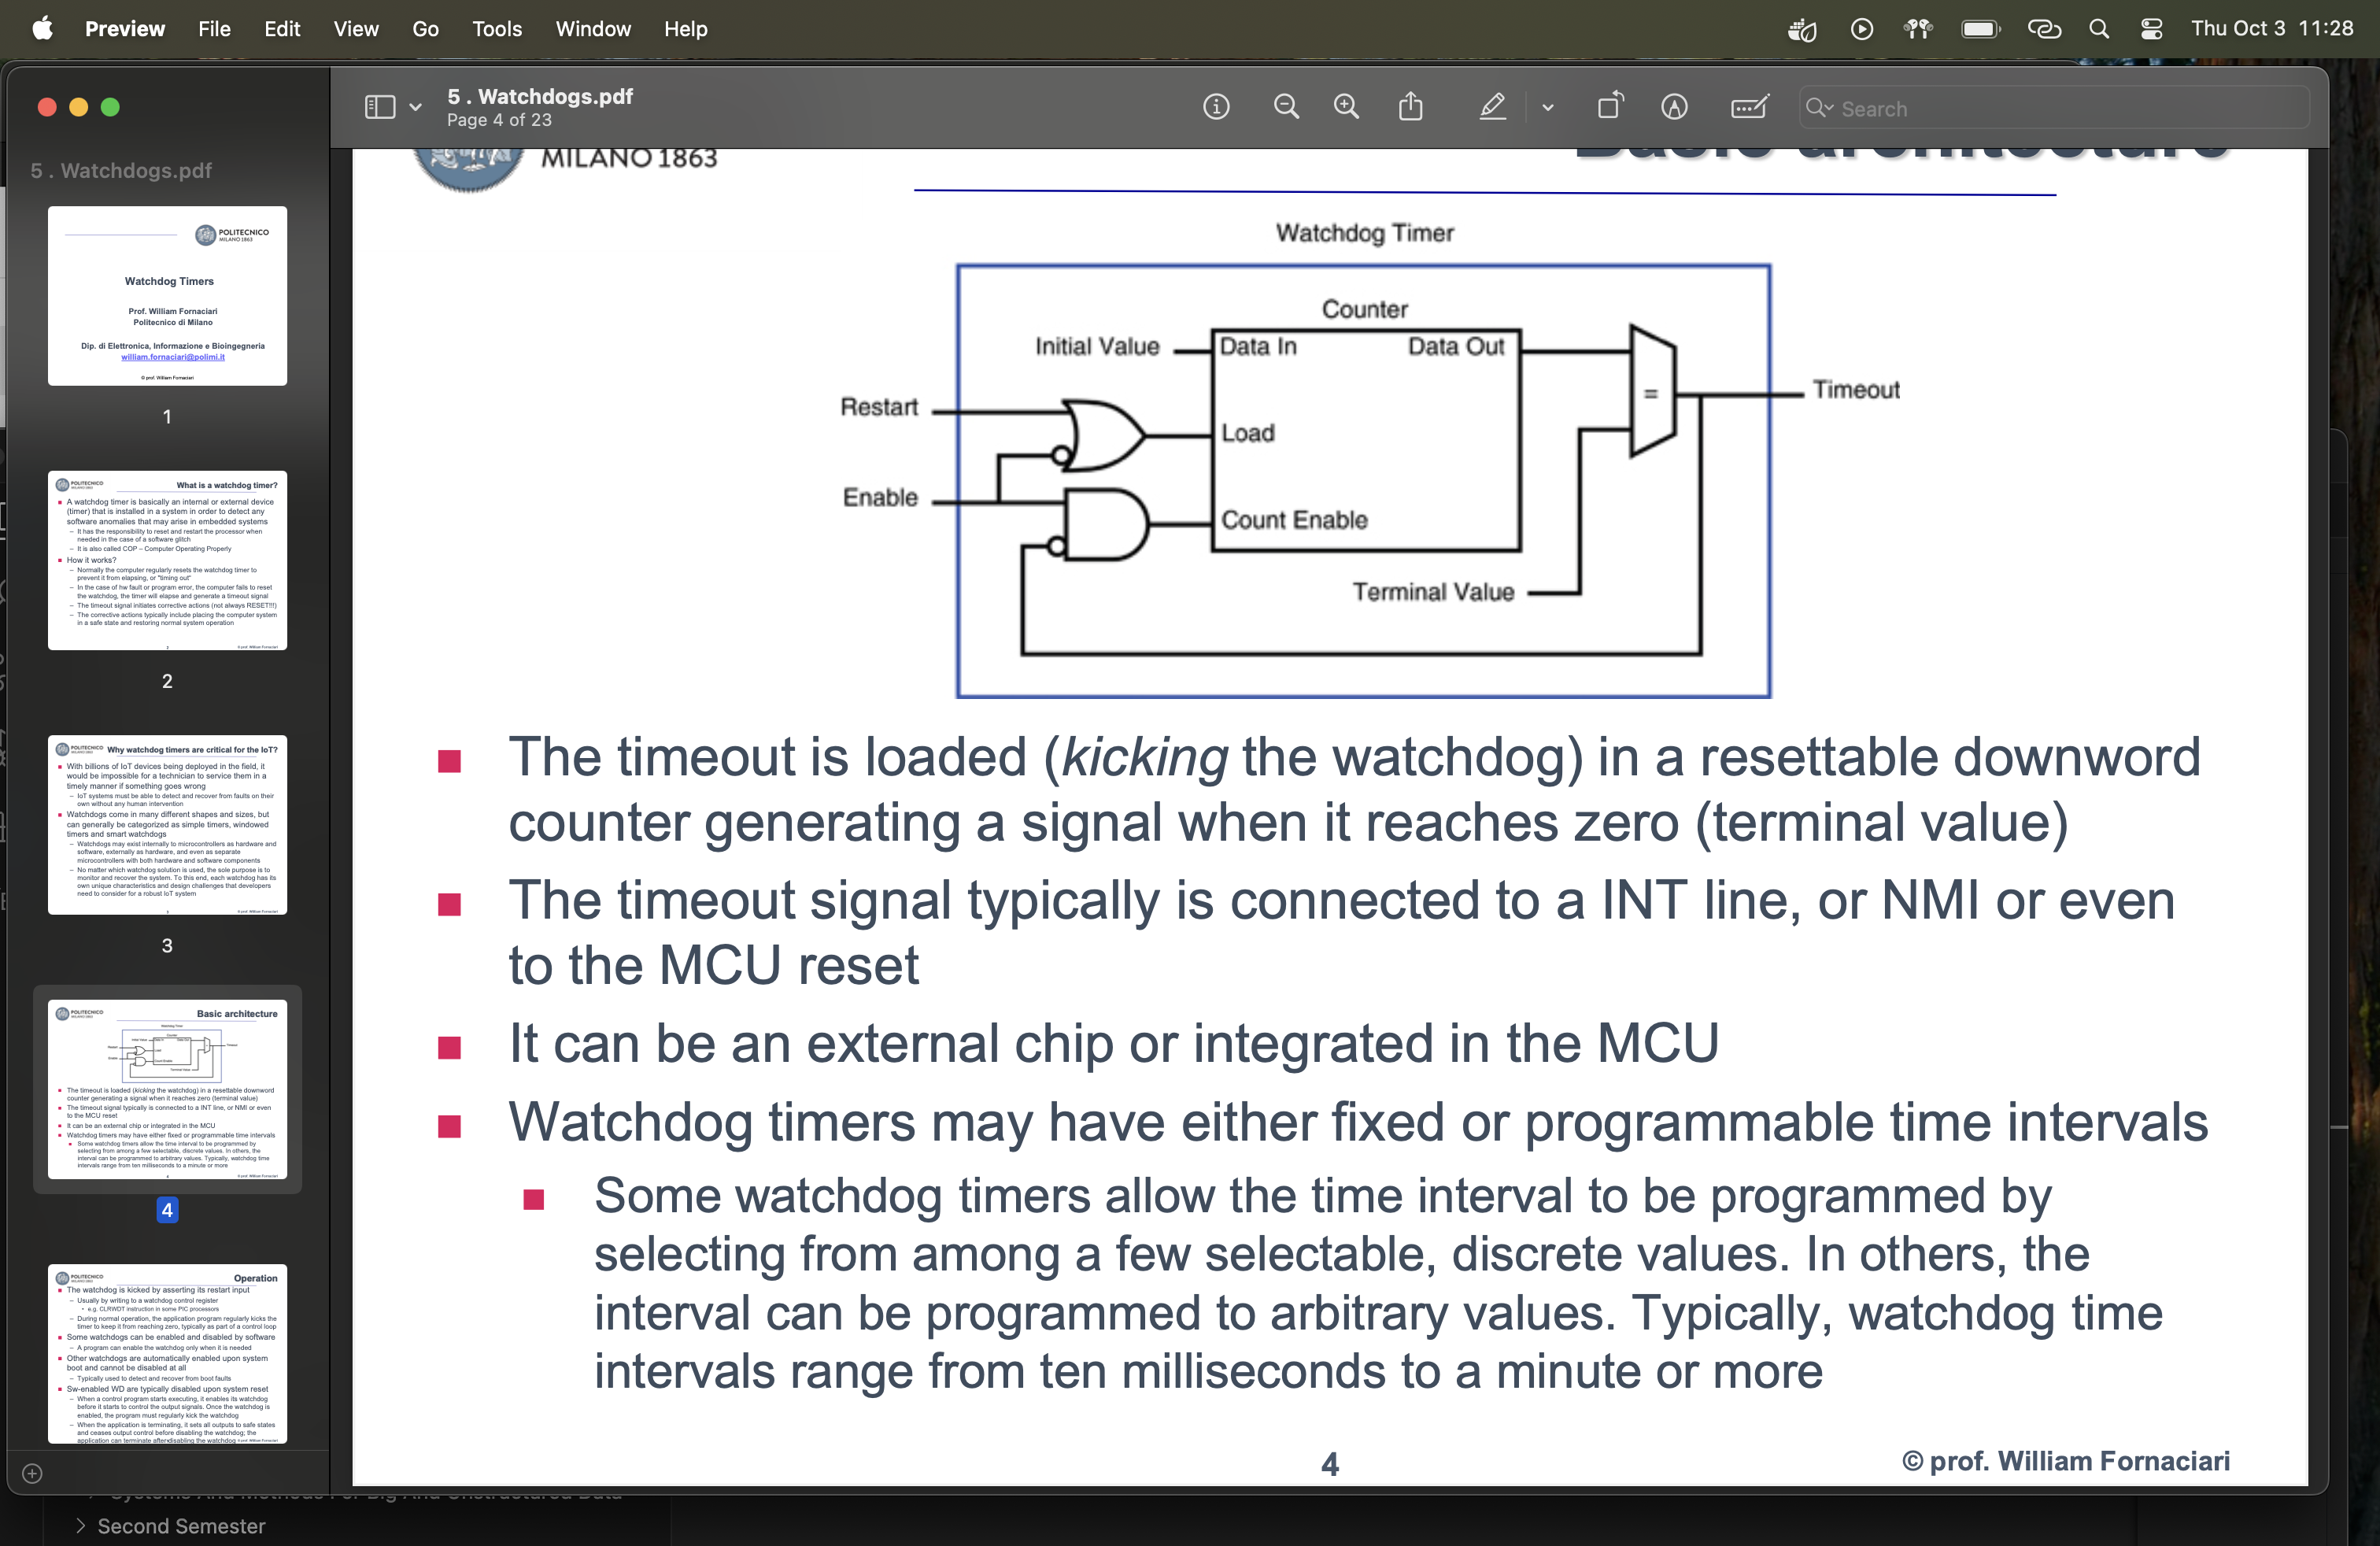
\includegraphics[width=0.75\linewidth]{images/wdog.png}
    \caption{Watchdogs architecture}
\end{figure}
The timeout is loaded (kicking the watchdog) in a resettable downword
counter generating a signal when it reaches zero (terminal value)
 The timeout signal typically is connected to a INT line, or NMI or even
to the MCU reset
 It can be an external chip or integrated in the MCU
 Watchdog timers may have either fixed or programmable time intervals
 Some watchdog timers allow the time interval to be programmed by
selecting from among a few selectable, discrete values. In others, the
interval can be programmed to arbitrary values. Typically, watchdog time
intervals range from ten milliseconds to a minute or more


The watchdog is kicked by asserting its restart input
– Usually by writing to a watchdog control register
• e.g. CLRWDT instruction in some PIC processors
– During normal operation, the application program regularly kicks the
timer to keep it from reaching zero, typically as part of a control loop
 Some watchdogs can be enabled and disabled by software
– A program can enable the watchdog only when it is needed
 Other watchdogs are automatically enabled upon system
boot and cannot be disabled at all
– Typically used to detect and recover from boot faults
 Sw-enabled WD are typically disabled upon system reset
– When a control program starts executing, it enables its watchdog
before it starts to control the output signals. Once the watchdog is
enabled, the program must regularly kick the watchdog
– When the application is terminating, it sets all outputs to safe states
and ceases output control before disabling the watchdog; the
application can terminate after disabling the watchdog

In case of problems Two corrective actions exists
– (1) Set of the MCU control outputs to safe levels so that potentially
dangerous devices such as motors and heaters will not pose threats
to people or equipment. High priority action that must occur as soon
as a fault is detected
– (2) After setting the outputs to safe levels restore normal system
operation
• This can be as simple as restarting the computer, as if a human
operator has pressed the computer’s reset pushbutton, or it may
involve a sequence of actions that ultimately ends with a computer
restart
• A watchdog timer can respond to faults more quickly than a human
operator, making it invaluable in cases where a human operator would
be too slow to react to a fault condition
• Watchdog timers may also be used when running untrusted code in a
sandbox, to limit the CPU time available to the code and thus prevent
some types of denial-of-service (DoS) attacks


\subsection{Single stage watchdog}
Single timer that invokes an immediate restart upon timeout
– The timeout signal is connected to the computer’s system reset
input, either directly or through a conditioning circuit, so that a
computer restart will occur when the watchdog times out
– This architecture depends on the system reset to force control
outputs to their safe states
• Some computers will power-down if a continuous timeout signal is
applied to the system reset input. In such cases, a pulse may be
required to initiate a system restart. A pulse generator can often be
used to satisfy this requirement
• MCU and watchdog may share the same clock signal
\begin{figure}[H]
    \centering
    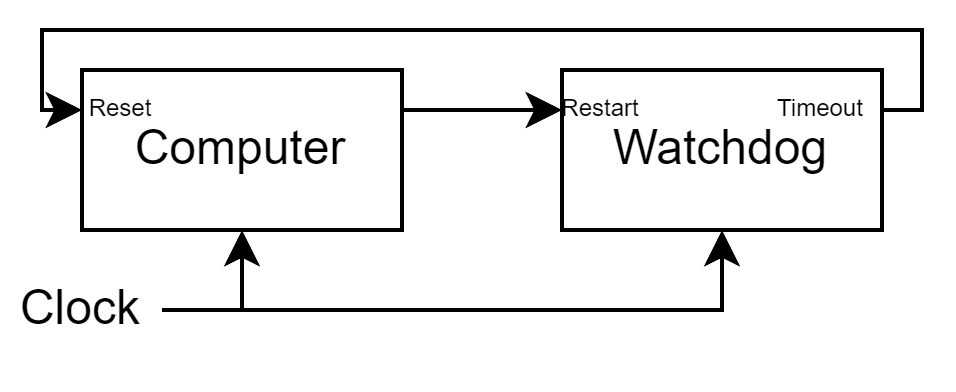
\includegraphics[width=0.75\linewidth]{images/swdog.png}
    \caption{Single stage watchdog}
\end{figure}

\subsection{Multiple stage watchdog}
Two or more timers cascaded to form a multistage
watchdog timer. Only the first stage is kicked by the
processor
– Upon first stage timeout, a corrective action is initiated and the next
stage in the cascade is started. As each subsequent stage times
out, it triggers a corrective action and starts the next stage
– Upon final stage timeout, a corrective action is initiated, but no other
stage is started because the end of the cascade has been reached
– Typically, single-stage watchdog timers are used to simply restart
the computer, whereas multistage watchdog timers will sequentially
trigger a series of corrective actions, with the final stage triggering a
computer restart
\begin{figure}[H]
    \centering
    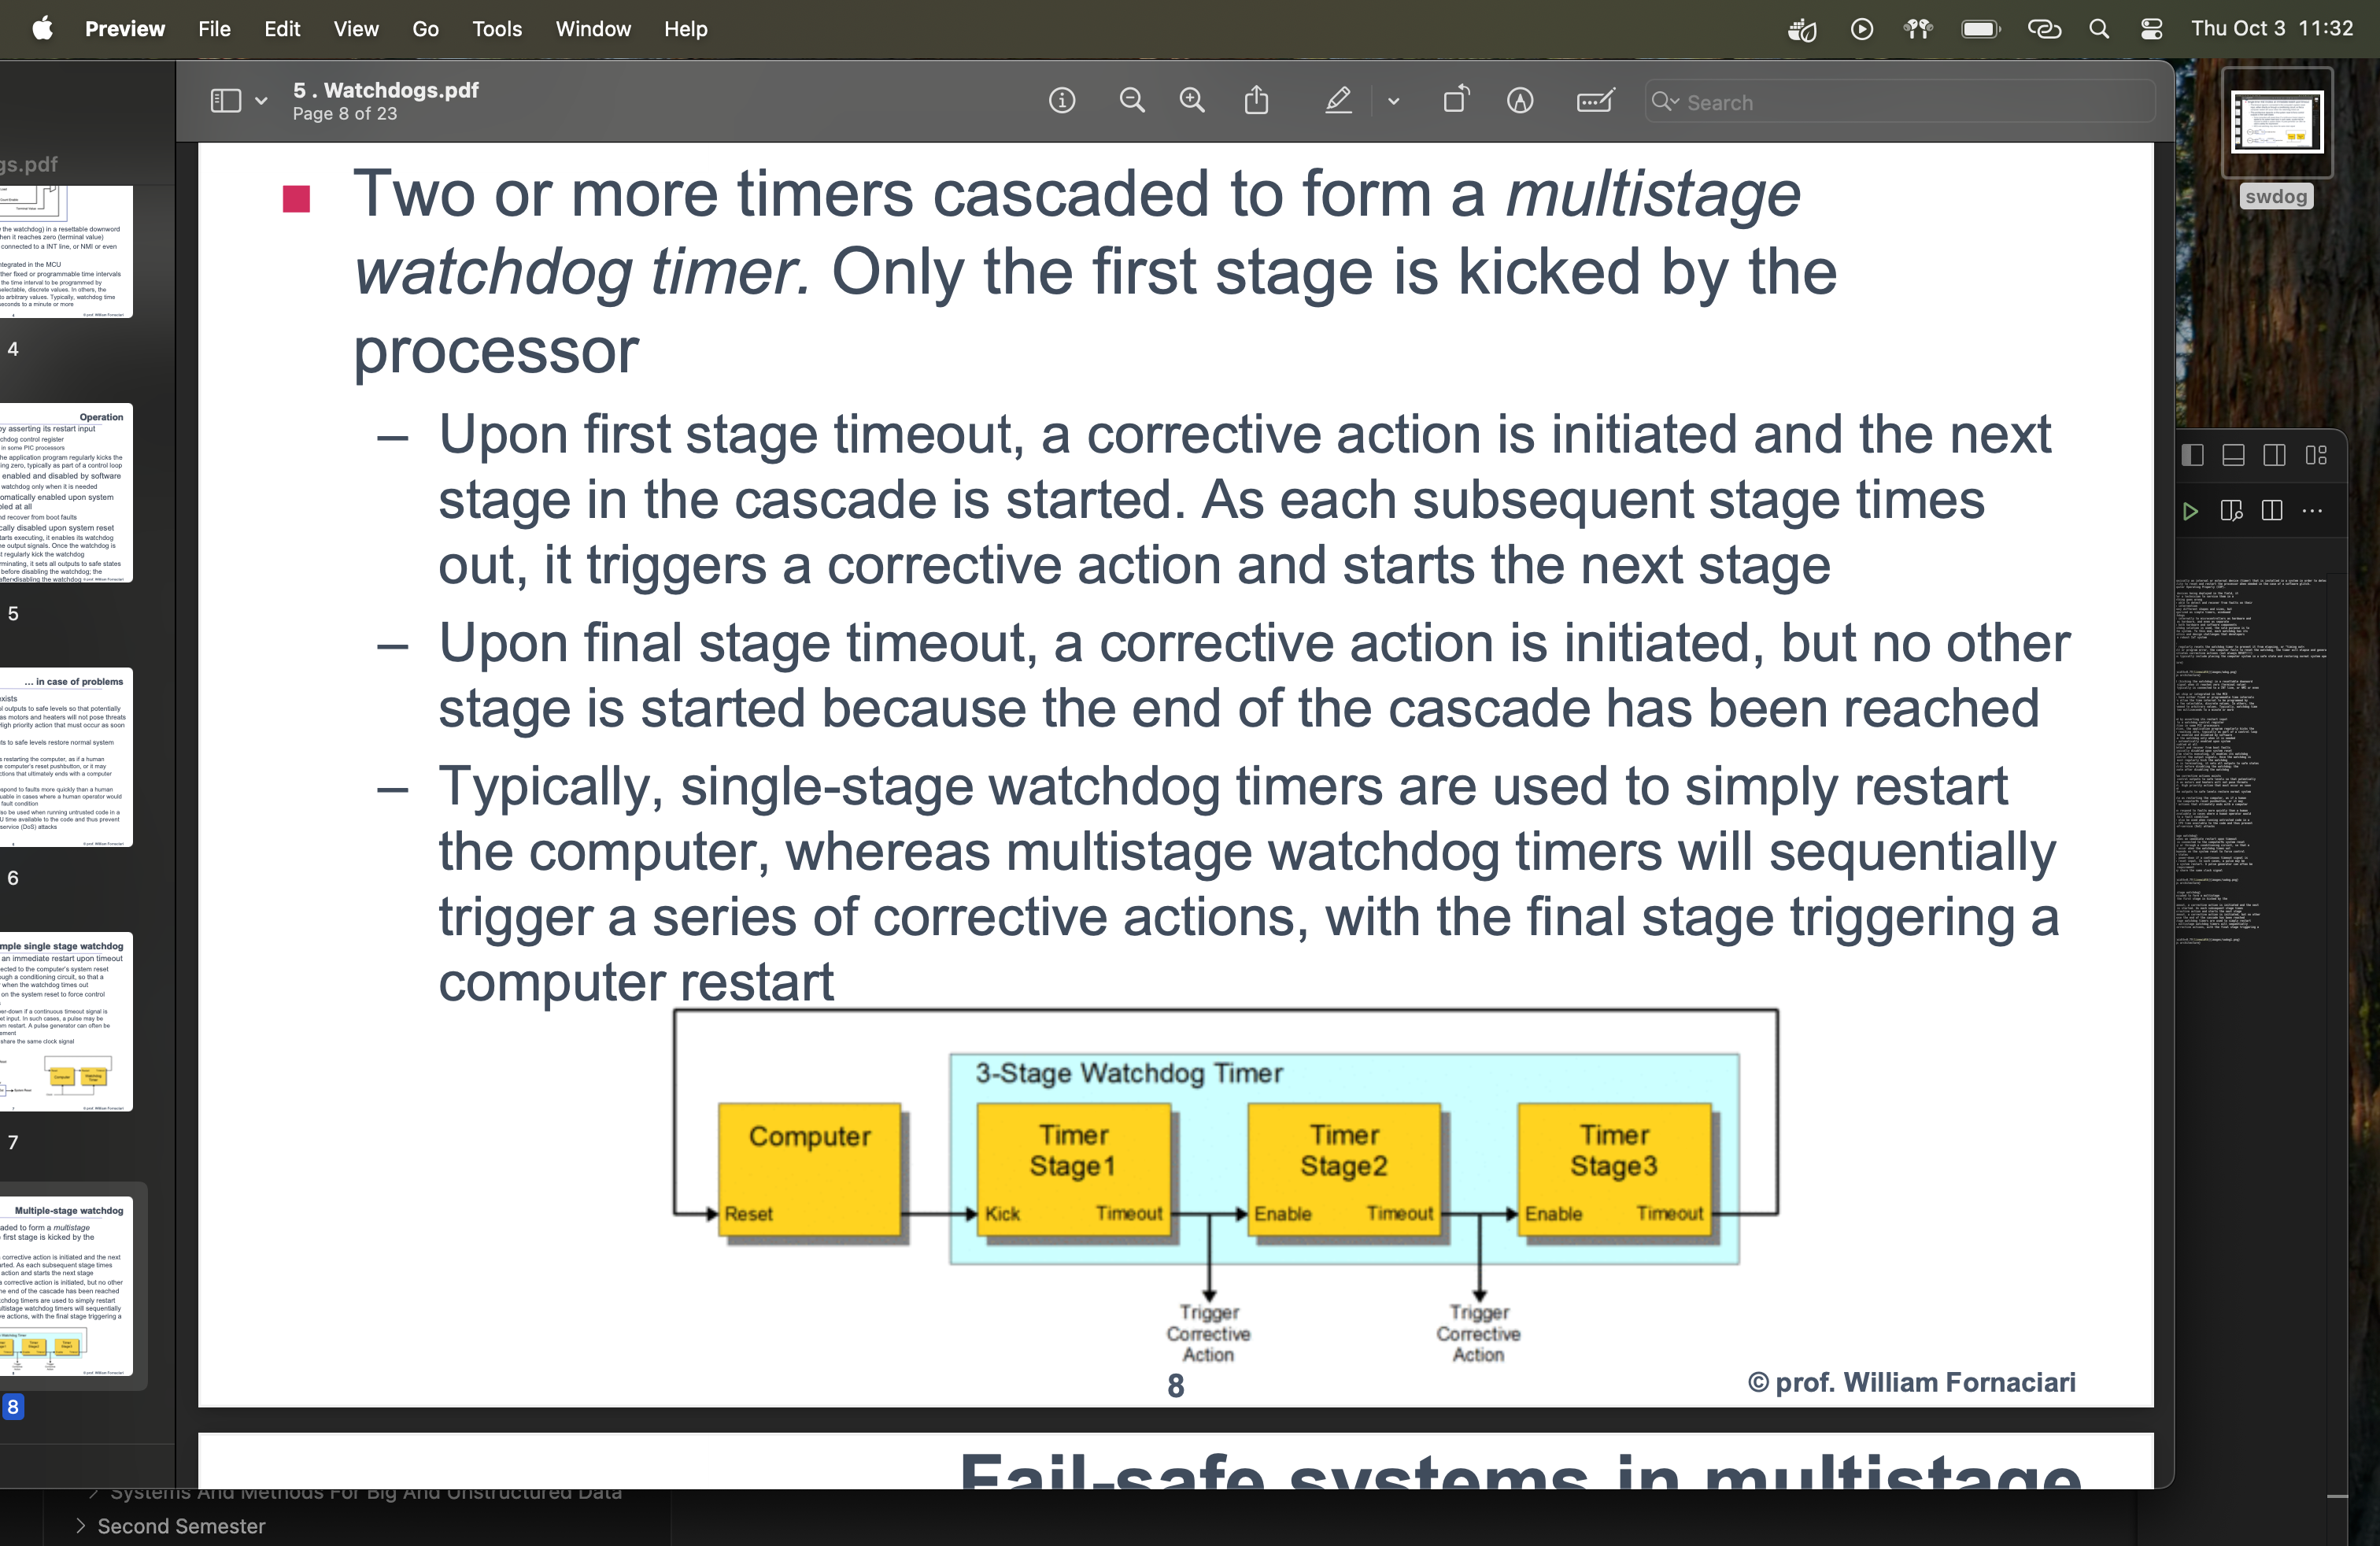
\includegraphics[width=0.75\linewidth]{images/swdog1.png}
    \caption{Multiple stage watchdog}
\end{figure}
Multistage watchdog timeout doesn’t immediately restart
MCU; it merely schedules a restart to occur at a future time
 A multistage watchdog must work in concert with special
circuitry that will switch outputs to safe states upon timeout,
prior to the computer/MCU restart
One way to do this is to employ a dedicated control reset signal that resets the control circuitry (but not the computer) upon watchdog timeout. 
This is easily implemented but it presents some complications and shortcomings:
Also, a reset can cause the loss of important state information needed for fault recovery, and it may interfere with the operation of interfaces that could otherwise continue to function normally during a fault condition

\paragraph*{Run mode and Safe mode}
The program can modify Runmode states at any time, but it can
change Safemode states only when permitted by a special write-
protect mechanism. Typically, the program will begin to control the
Runmode states after it establishes Safemode states, which
comprise a complete, customized set of safe states for all outputs
– During normal operation, the Runmode states are routed through
the data selector to the outputs. Upon watchdog timeout, the data
selector switches input sets so that Safemode states are applied to
the outputs in place of Runmode states. Since the control circuitry
has not been reset, it will continue to function normally (to the
extent possible) and it will retain interface state information (e.g.,
incremental encoder counts, captured events, hardware
configuration) that may be needed for fault recovery
\begin{figure}[H]
    \centering
    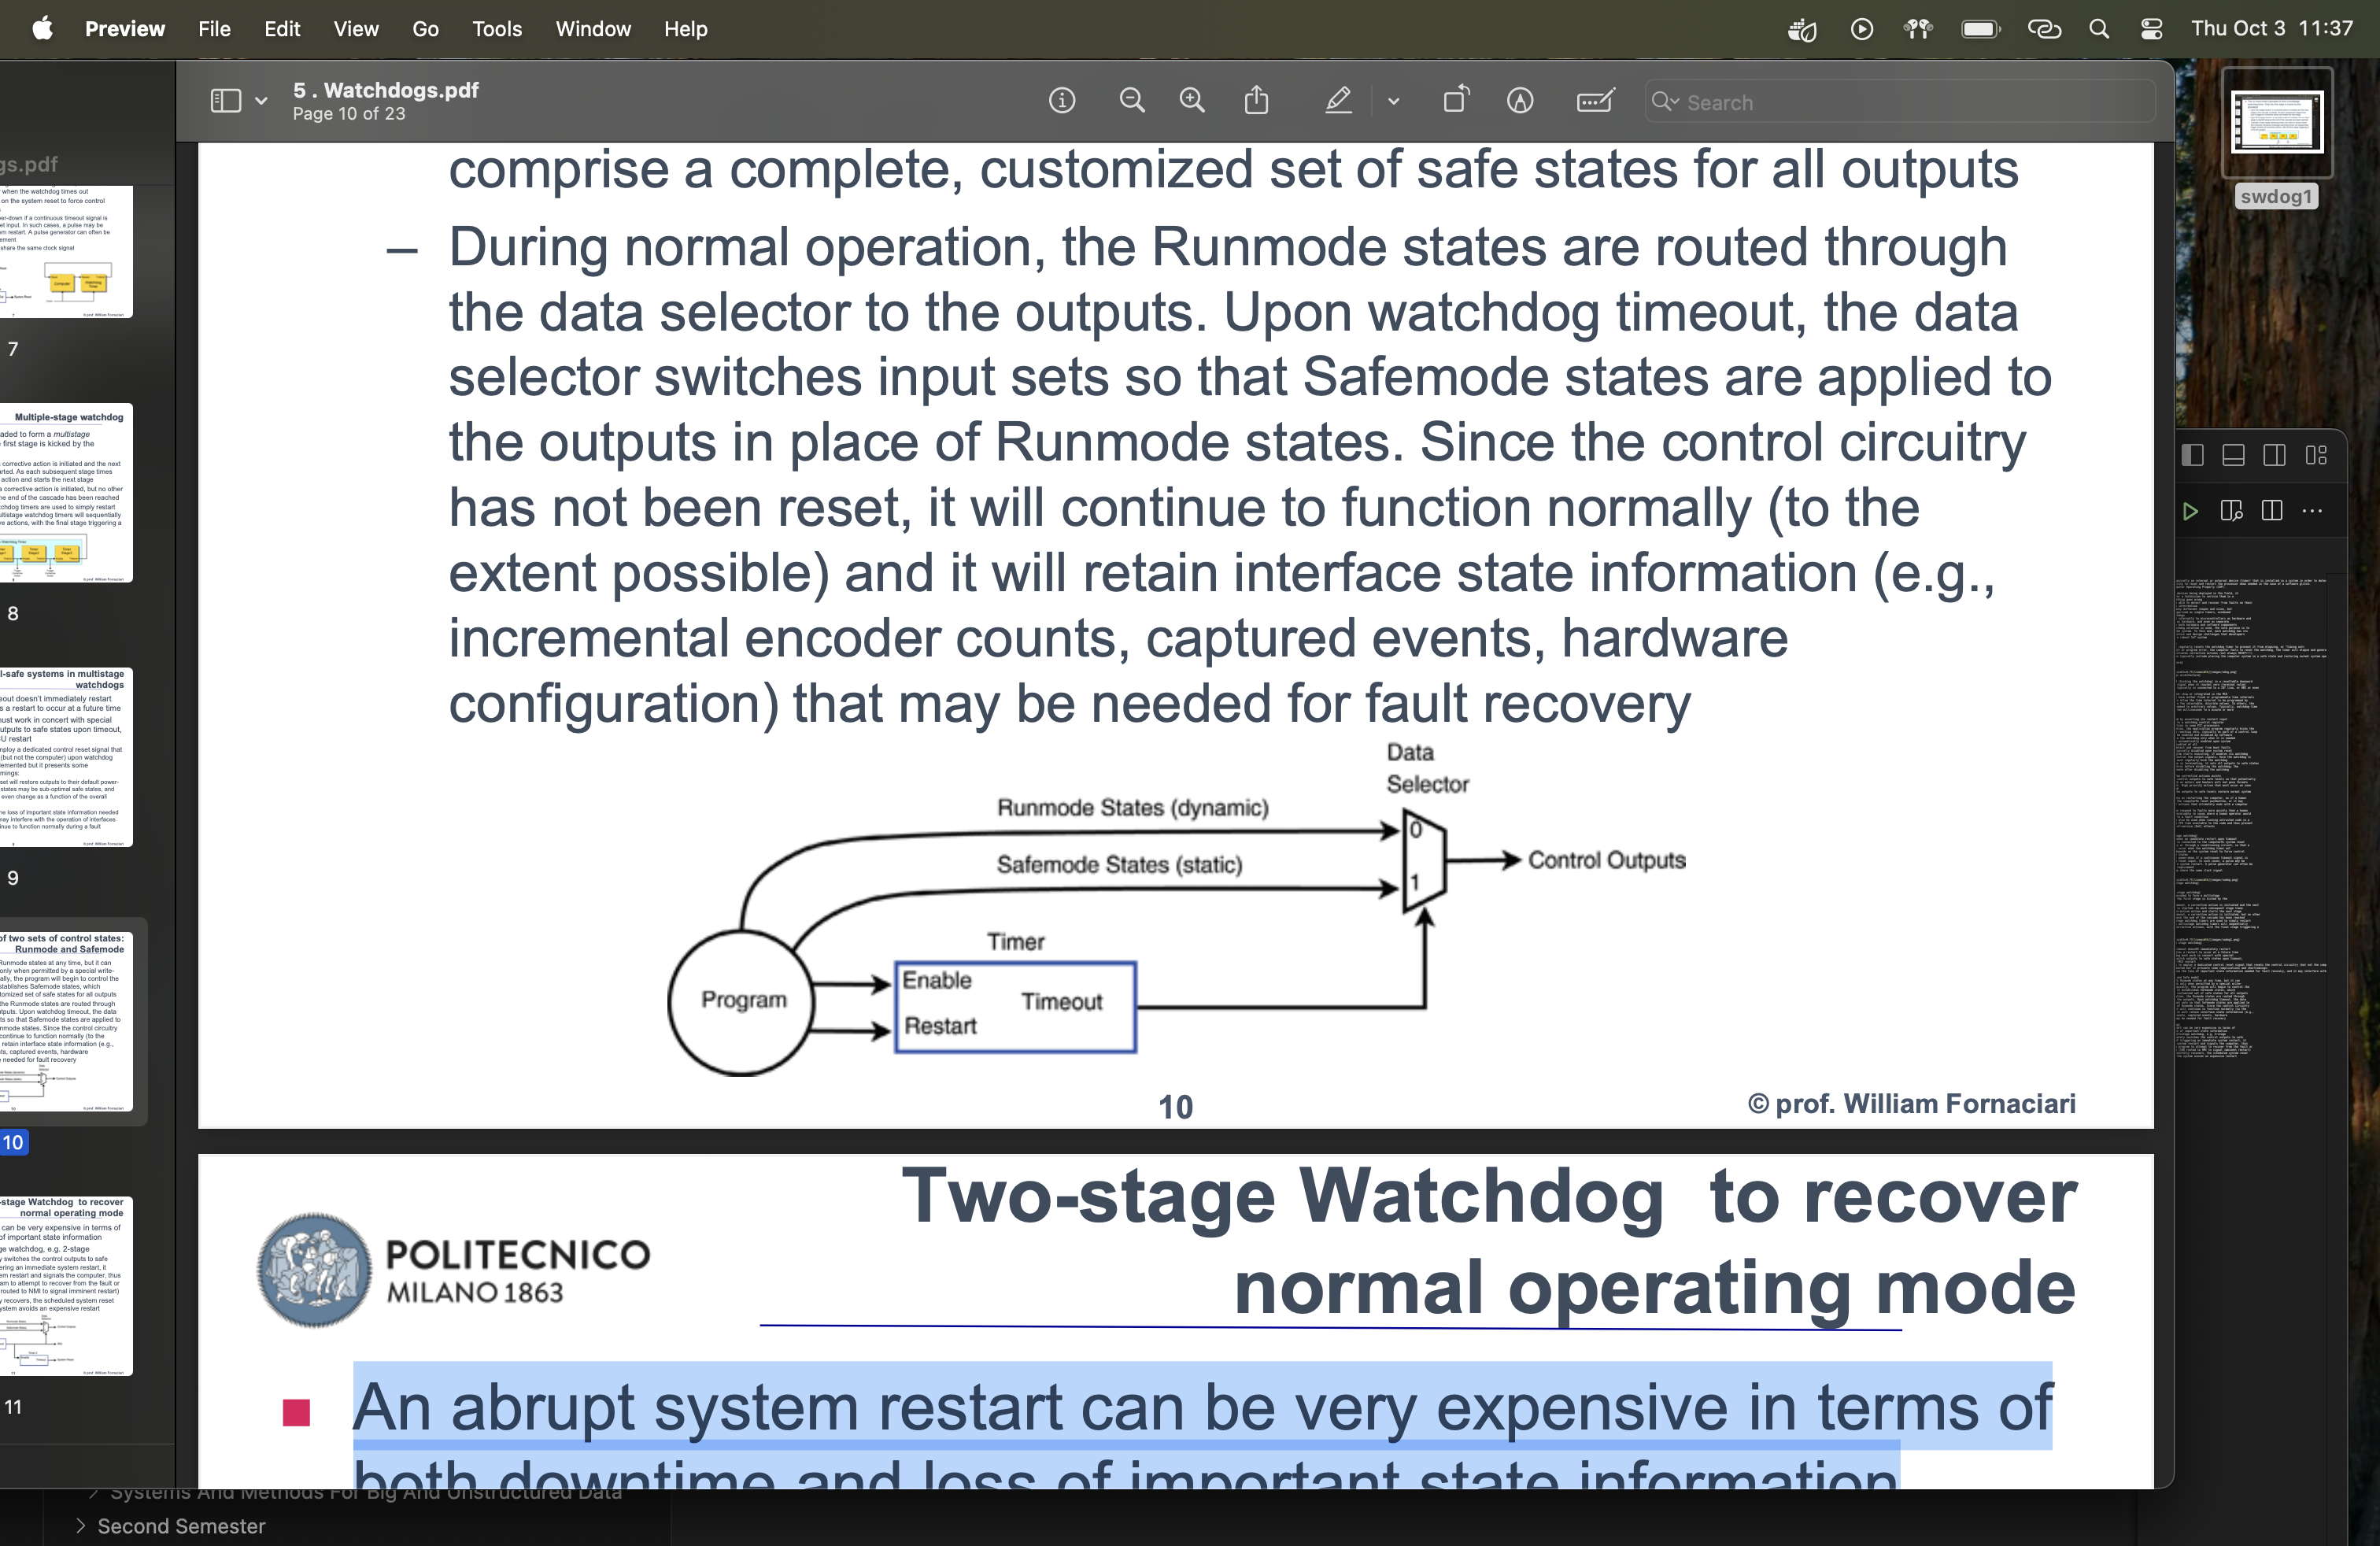
\includegraphics[width=0.75\linewidth]{images/wdog1.png}
    \caption{Watchdog mode}
\end{figure}

\paragraph*{Recovering}
An abrupt system restart can be very expensive in terms of
both downtime and loss of important state information
 Mitigated with a multistage watchdog, e.g. 2-stage
– The watchdog immediately switches the control outputs to safe
states, but instead of triggering an immediate system restart, it
schedules a deferred system restart and signals the computer, thus
allowing time for the program to attempt to recover from the fault or
log state information (IRQ routed to NMI to signal imminent restart)
– If the program successfully recovers, the scheduled system reset
will be canceled and the system avoids an expensive restart
\begin{figure}[H]
    \centering
    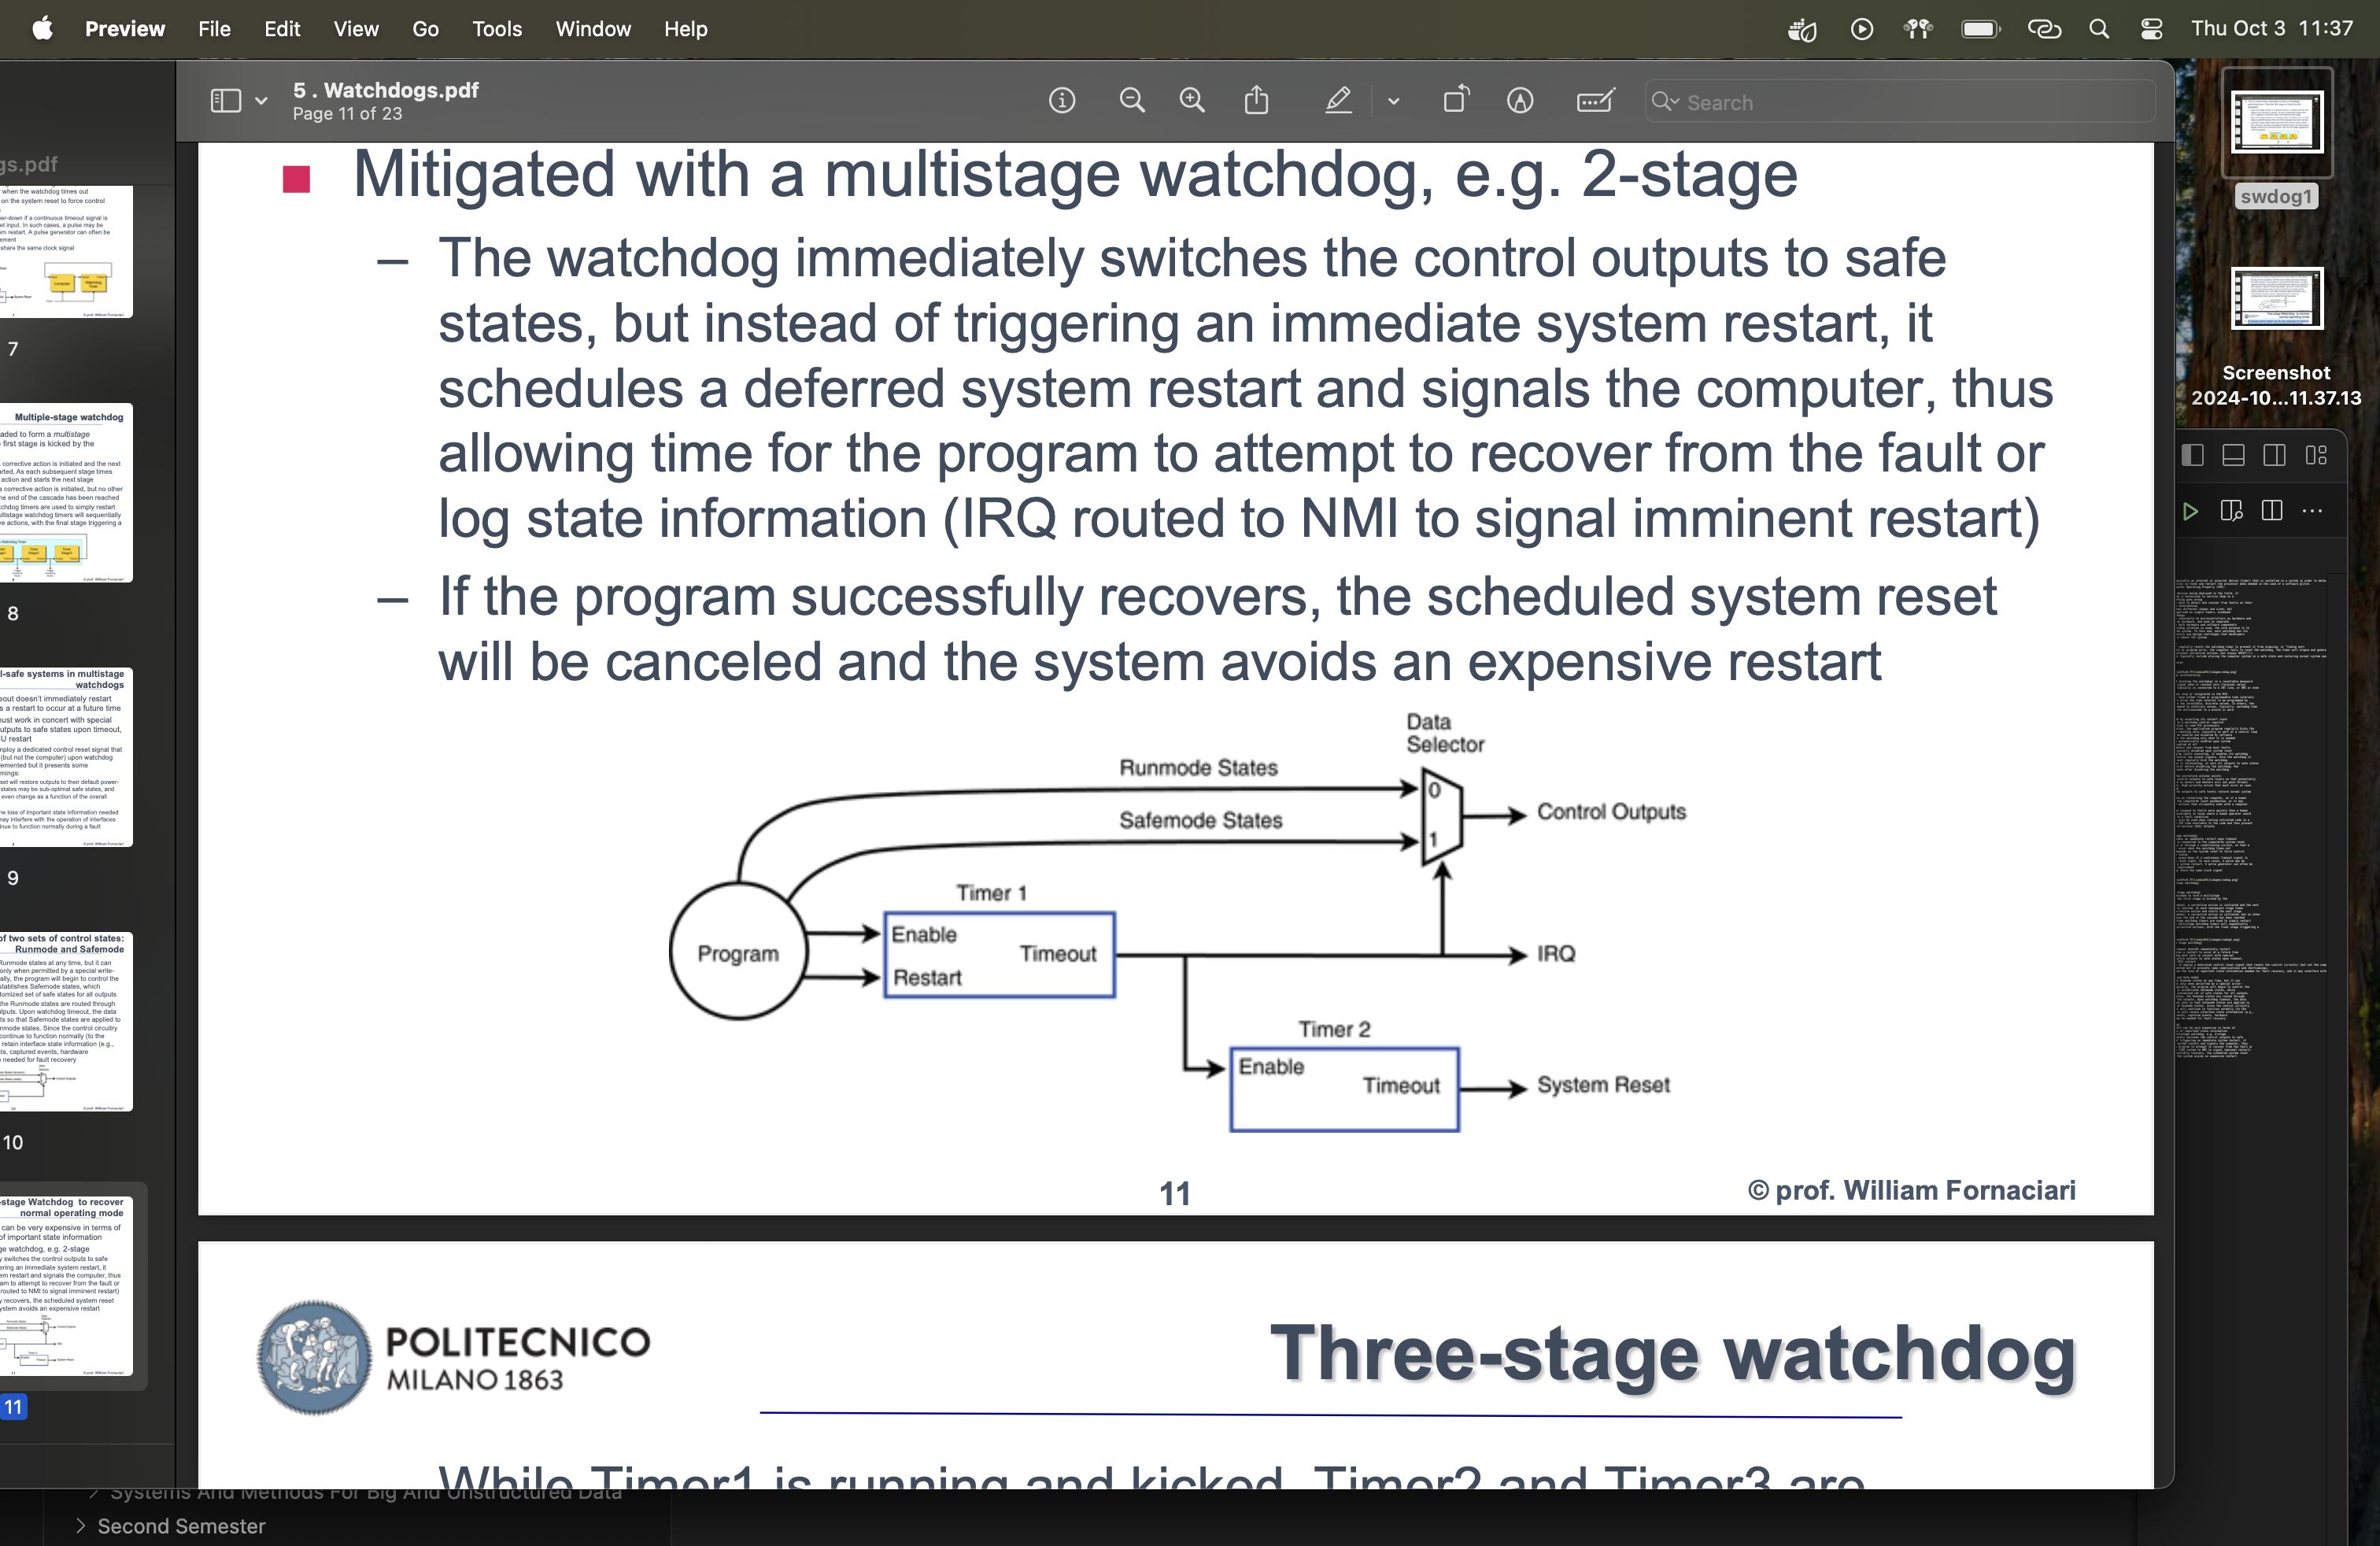
\includegraphics[width=0.75\linewidth]{images/wdog2.png}
    \caption{Watchdog recovery}
\end{figure}

\subsection{Three-stage watchdog}
While Timer1 is running and kicked, Timer2 and Timer3 are
disabled and held at their initial values and the control outputs are
allowed to change under program control
– Timer1 timeout will switch the outputs to safe states, start Timer2,
and requests interrupt service. If the computer is able to respond to
the IRQ, the program will attempt to recover from the fault condition
and, if successful, the program will disable Timer1 (and by
extension, Timer2), thus canceling further corrective actions
– If the computer cannot
respond to the IRQ
• Timer2 will timeout, start
Timer3 and assert a NMI
to indicate imminent
system restart
• Make possible logging
important fault
information (e.g., crash
dump) before restart
\begin{figure}[H]
    \centering
    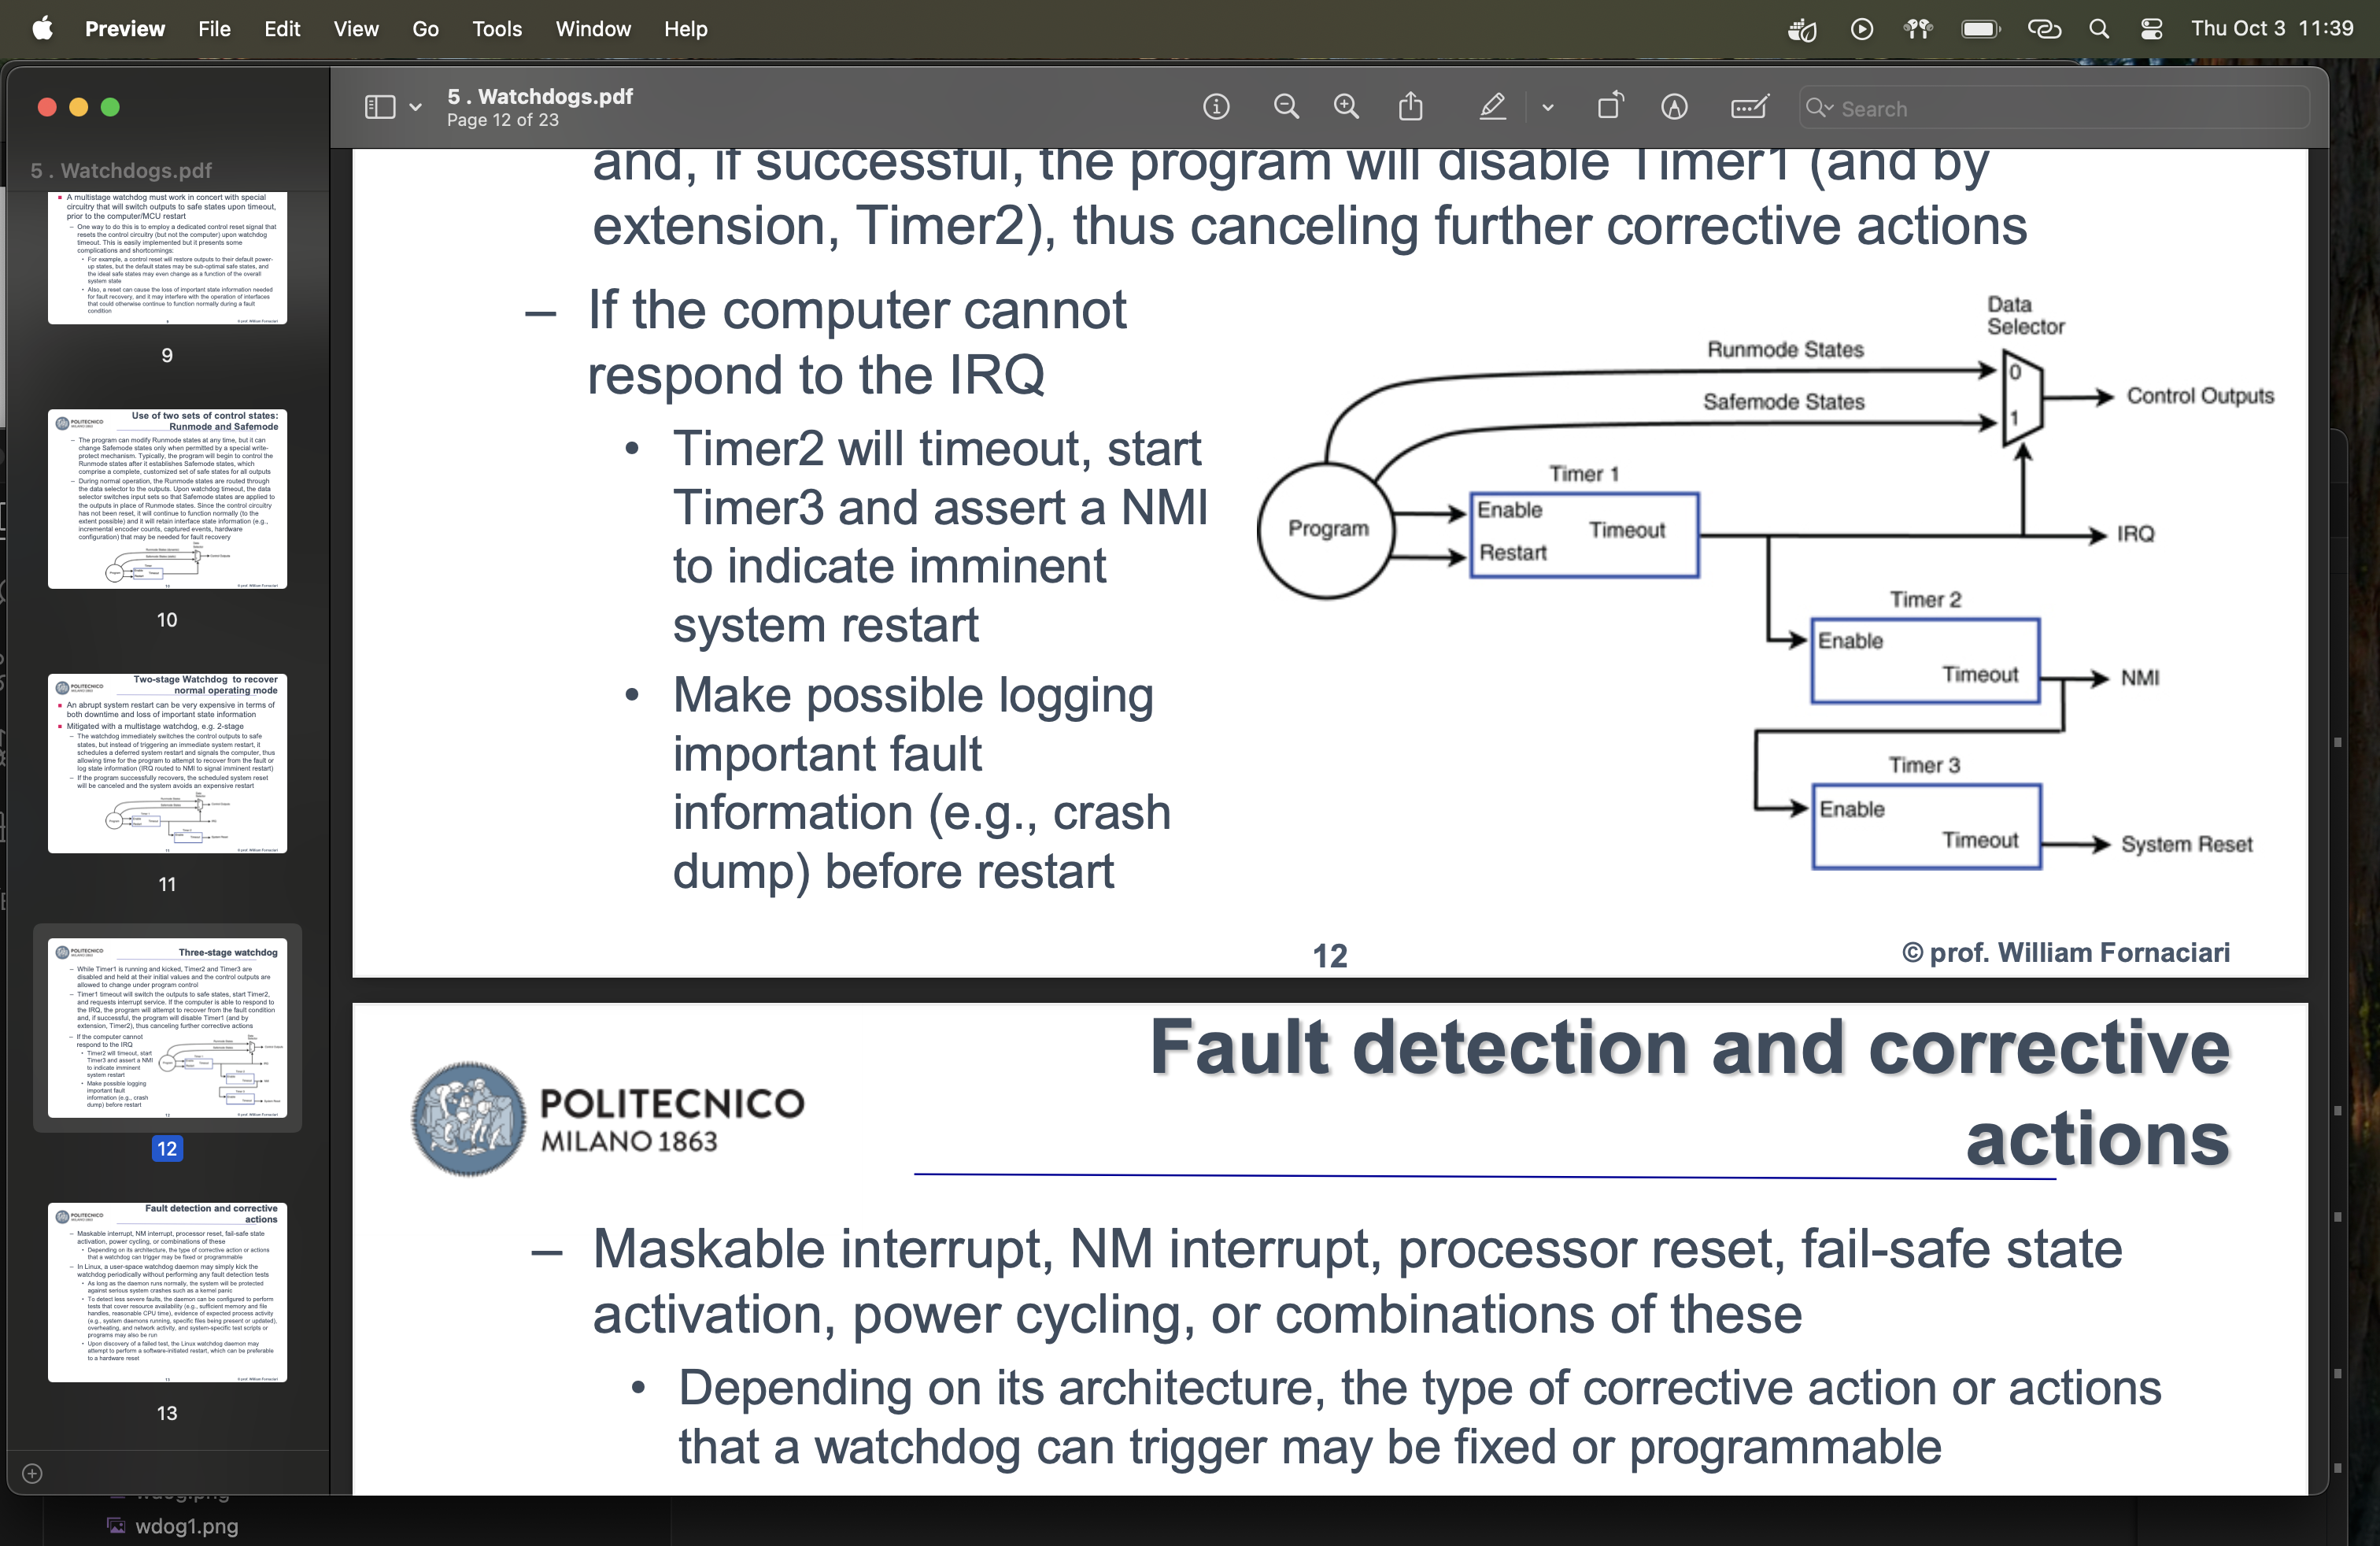
\includegraphics[width=0.75\linewidth]{images/wdog3.png}
    \caption{Three-stage watchdog}
\end{figure}

\paragraph*{Fault detection}
Maskable interrupt, NM interrupt, processor reset, fail-safe state
activation, power cycling, or combinations of these
• Depending on its architecture, the type of corrective action or actions
that a watchdog can trigger may be fixed or programmable
– In Linux, a user-space watchdog daemon may simply kick the
watchdog periodically without performing any fault detection tests
• As long as the daemon runs normally, the system will be protected
against serious system crashes such as a kernel panic
• To detect less severe faults, the daemon can be configured to perform
tests that cover resource availability (e.g., sufficient memory and file
handles, reasonable CPU time), evidence of expected process activity
(e.g., system daemons running, specific files being present or updated),
overheating, and network activity, and system-specific test scripts or
programs may also be run
• Upon discovery of a failed test, the Linux watchdog daemon may
attempt to perform a software-initiated restart, which can be preferable
to a hardware reset

\subsection{AVR watchdog}
AVR® devices have an Enhanced Watchdog Timer (WDT)
that runs on a separate oscillator from the main clock
– WDT is essentially a counter that increments based on the clock
cycles of an on-chip 128kHz oscillator
– The WDT forces an interrupt or a system reset when the counter
reaches a given time-out value
– Selectable Time-out period from 16 milliseconds to 8 seconds
In normal operation mode, the
application code needs to issue
a Watchdog Timer Reset
(WDR) instruction to restart the
counter before the time-out
value is reached. If the system
doesn't restart the counter, an
interrupt or system reset will be
issued
Three operating modes
– Interrupt Mode
• WDT forces an interrupt when the timer expires. This interrupt can be
used to wake the device from any of the sleep-modes, and also as a
general system timer. One example is to limit the maximum time
allowed for certain operations, forcing an interrupt when the operation
has run longer than expected. This is enabled by setting the Interrupt
mode bit (WDIE) in the Watchdog Timer Control Register (WDTCSR)
– System Reset
• WDT forces a reset when the timer expires. This is typically used to
prevent system hang-up in the case of runaway code. This is enabled
by setting the System Reset mode bit (WDE) in the Watchdog Timer
Control Register (WDTCSR)
– Interrupt and System Reset Mode
• Interrupt and System Reset mode combines the other two modes by
first forcing an interrupt and then switching to the System Reset mode.
This mode will offer a safe shutdown by allowing time to save critical
parameters before a system reset. This is enabled when both the
WDTIE and WDTE are set

\subsection{Watchdogs usage}
– Never disable the watchdog for any reason
– Never clear the watchdog in a periodic interrupt independent from
software functionality checks
– Verify that the watchdog timer is an independent watchdog.
Independent watchdogs have a separate clock that allows them to
detect if the system clock has halted
– Use a watchdog that has a windowed watchdog feature
• These watchdogs require a minimum time before the watchdog can be
cleared. If an attempt is made prior to the start of the window, the
watchdog will reset the system. This prevents runaway software from
overriding the watchdog timer
– Internal WDT are a good step towards building a robust embedded
system, but on their own they don’t provide a very robust solution
• In order to really up the ante with respect to robustness, developers
need to consider external watchdogs

\subsection{External watchdogs}
Many internal implementations have flaws
– Examples are sharing the system clock, and having a disable option
 External watchdog has many advantages, such as
– Performing a hard system reset that ensures the microcontroller is
power cycled, which in turn power cycles the internal peripherals
– Separating the watchdog from the microcontrollers oscillator circuit
– Providing a completely independent process for monitoring the
system
 All of these contribute to system robustness, although there
are also a few disadvantages to using an external WDT
– Increase in hardware costs due to the addition of an IC as well as
an increase in system complexity


\subsection{Smart watchdogs}
A smart watchdog is a supervisory microcontroller that, in
addition to performing basic heartbeat monitoring, can also
monitor system communications
– There can be instances where the microcontroller stops responding
to the Internet, but is still successfully clearing the external
watchdog
– When this happens, a command could be sent over the Internet to
reset the microcontroller
– The smart watchdog can monitor the communication lines, such as
UART transmit and receive lines, for a special command that tells it
to restart the system
– There are several mic


